\documentclass[12pt, a4paper, oneside, openany,DIV=16 headings=small]{scrbook}

% Eingelagerte Präambel
% Sprach-/Font-Setup
\usepackage[T1]{fontenc}
\usepackage[utf8]{inputenc}
\usepackage[ngerman]{babel}
\usepackage{lmodern}
\usepackage{microtype}
\usepackage{csquotes}
\usepackage{changepage}
\usepackage{listings}
\usepackage{listingsutf8}

% Mathe & Physik
\usepackage{amsmath, amssymb, amsthm, tcolorbox}
\usepackage{siunitx}     % \SI{...}{...}
\sisetup{locale=DE, per-mode=symbol}
\usepackage{physics}     % \dv, \grad, \laplacian etc. (optional)

% Grafik, Tabellen
\usepackage{graphicx}
\usepackage{subcaption}
\usepackage{booktabs}
\usepackage{array}
\usepackage{tikz}
\usepackage{pgfplots}
\pgfplotsset{compat=newest}

% Referenzen/Links
\usepackage[hidelinks]{hyperref}
\usepackage[capitalise,noabbrev]{cleveref}

% Code-Listings (ohne shell-escape)
\usepackage{listings}
\lstset{
  basicstyle=\ttfamily\small,
  frame=single,
  numbers=left,
  numberstyle=\tiny,
  breaklines=true,
  tabsize=2,
  language=Python
}

% Bibliographie
\usepackage[
  backend=biber,
  style=authoryear,
  giveninits=true,
  maxcitenames=2, maxbibnames=20,
  uniquename=false, sorting=nyt,
  doi=false, isbn=false, url=false
]{biblatex}

\addbibresource{bib/references.bib}

% --- Glossar ---
%\usepackage{glossaries-extra}
%\setabbreviationstyle[acronym]{long-short}
%\makeglossaries

% Einfache, saubere Makros
\newcommand{\alphastar}{\ensuremath{\alpha^{\ast}}}
\newcommand{\ERTh}{Energie-Resonanz-Theorie}
\newcommand{\helm}{Helmholtz-Gleichung}
\newcommand{\robin}{Robin-Randbedingung}

% Vektor/Laplace etc. (falls physics nicht genutzt wird)
% \newcommand{\laplace}{\nabla^2}

% Einheiten-Kürzel
\newcommand{\GB}{\ensuremath{\,\mathrm{GB}}}
\newcommand{\EB}{\ensuremath{\,\mathrm{EB}}}

% Abstract-Umgebung für scrbook definieren
\providecommand{\abstractname}{Zusammenfassung}
\makeatletter
\newenvironment{abstract}{%
  \cleardoublepage
  \chapter*{\abstractname}%
  \addcontentsline{toc}{chapter}{\abstractname}%
  \markboth{\abstractname}{\abstractname}%
}{\par}
\makeatother

% Lockerere Float-Regeln
\makeatletter
\renewcommand{\topfraction}{0.95}      % Anteil oben: bis 95% Float erlaubt
\renewcommand{\bottomfraction}{0.95}   % Anteil unten: bis 95% Float
\renewcommand{\textfraction}{0.01}     % Mindesttextanteil auf Seite: nur 5%
\renewcommand{\floatpagefraction}{0.5}
\setcounter{topnumber}{3}              % max. Floats oben
\setcounter{bottomnumber}{2}           % max. Floats unten
\setcounter{totalnumber}{5}            % max. Floats gesamt pro Seite
\makeatother

% (optional, für engere Abstände)
\setlength{\textfloatsep}{10pt plus 2pt minus 2pt}
\setlength{\intextsep}{10pt plus 2pt minus 2pt}

% - Benutzung im Text:
%   \gls{alpha-star}, \Gls{spiralis}, \acrshort{ERT}, \acrlong{ART} etc.

% Haupt-Begriffe

\newglossaryentry{alpha-star}{%
  name={\ensuremath{\alpha^\star}},
  sort={alpha-star},
  text={\ensuremath{\alpha^\star}},
  description={%
    Dimensionsloser Operator der Energie–Zeit–Abweichung zur idealen Periode; in der ERT der \emph{Öffnungswinkel} der realen Spiraldynamik. %
    \ensuremath{\alpha^\star} legt die aperiodische Phasenverschiebung fest und bestimmt damit Resonanz, Skalenkopplung und Wahrnehmungsrahmen.},
  plural={\ensuremath{\alpha^\star}}%
}

\newglossaryentry{spiralis}{%
  name={Spiralis},
  sort={spiralis},
  description={%
    Erweiterung der Sinusfunktion zur \emph{dreidimensionalen, aperiodischen} Felddynamik. %
    Die Spiralis erzeugt aus drei dualen Raumrichtungen ein fraktales, resonantes Feld, dessen Zeitverlauf als geometrische Folge erscheint.},
  plural={Spirales}%
}

\newglossaryentry{aperiodizitaet}{%
  name={Aperiodizität},
  sort={aperiodizitaet},
  description={%
    Abwesenheit exakter Wiederkehr. In der ERT ist Aperiodizität eine essentielle Eigenschaft realer Dynamik: %
    Umlaufbahnen, Energieflüsse und Kopplungen schließen nicht exakt, sondern nähern sich asymptotisch periodischen Mustern an.}%
}

\newglossaryentry{resonanz}{%
  name={Resonanz},
  sort={resonanz},
  description={%
    Überlagerung kohärenter Wellenanteile mit Stabilisierung bestimmter Strukturen (Knoten/Zonen). %
    In der ERT entstehen so hierarchische Kopplungen (Proton $\rightarrow$ H $\rightarrow$ H$_2$ $\rightarrow$ H$^2$O).}%
}

\newglossaryentry{helmholtz}{%
  name={Helmholtz-Gleichung},
  sort={helmholtz},
  description={%
    Partielle Differentialgleichung, die stationäre Wellenfelder beschreibt. %
    In der ERT dient sie als Ausgangspunkt für das Eigenwertproblem im dreidimensionalen Randwert-Setup.}%
}

\newglossaryentry{robin}{%
  name={Robin-Randbedingung},
  sort={robin},
  description={%
    Lineare Randbedingung der Form \ensuremath{a u + b\,\partial_n u = c} an der Grenze des Lösungsgebiets. %
    In der ERT modelliert sie Energiefluss und Balance zwischen Feld und „Außenraum“.}%
}

\newglossaryentry{eigenwert}{%
  name={Eigenwert},
  sort={eigenwert},
  description={%
    Spektralbegriffe des Randwertproblems: Eigenwerte quantisieren zulässige Feldmodi; Eigenfunktionen sind die zugehörigen räumlichen Muster. %
    Der numerische Scan/ Fit der ERT identifiziert ein konsistentes Spektralsignal für \gls{alpha-star}.}%
}

\newglossaryentry{wahrnehmungsrahmen}{%
  name={Wahrnehmungsrahmen},
  sort={wahrnehmungsrahmen},
  description={%
    Effektive, periodische Maske menschlicher Messung und Erfahrung. %
    In der ERT wird Zeit als aus dem Feld emergierende Geometrie verstanden; der Wahrnehmungsrahmen begrenzt Sichtbarkeit (z.\,B. Lichtgeschwindigkeit, EM-Spektrum).}%
}

\newglossaryentry{dualitaet}{%
  name={Dualität (Richtungen)},
  sort={dualitaet},
  description={%
    Jede Raumdimension besitzt zwei Richtungen; Negativität wird nicht benötigt. %
    Die dreifache Dualität erzeugt acht erste Überlagerungspunkte (Ecken eines Würfels) als elementare Resonanzstruktur.}%
}

\newglossaryentry{achter-raster}{%
  name={8er-Raster},
  sort={achter-raster},
  description={%
    Diskretisierung entlang der acht kubischen Richtungen. %
    Dient im ERT-Scan als minimaler symmetrischer Suchraum, in dem Resonanzknoten zuverlässig detektierbar werden.}%
}

\newglossaryentry{hierarchie}{%
  name={Diadische Hierarchie},
  sort={hierarchie},
  description={%
    Skalierung/Einbettung von Resonanzknoten über Faktoren von zwei und acht, wodurch fraktale, selbstähnliche Strukturen über Skalen hinweg entstehen.}%
}

\newglossaryentry{normalisierung}{%
  name={Normalisierung},
  sort={normalisierung},
  description={%
    Abbildung der berechneten Felder auf \([0,1]\) zur Visualisierung. %
    Der Punkt \mbox{\(0{,}5\)} markiert die Wahrnehmungsnull (Raum), während \(\,1-\alpha^\star/10\,\) die sichtbare Informationsgrenze setzt.}%
}

\newglossaryentry{em-colormap}{%
  name={EM-Colormap (ERT)},
  sort={em-colormap},
  description={%
    Farbcodierung, die das sichtbare Spektrum (Violett\,$\to$\,Weiß) in Einklang mit \gls{alpha-star} abbildet, inkl.\ UV/IR-Interpretation als „Rand“-Informationen des Wahrnehmungsfensters.}%
}

\newglossaryentry{vti}{%
  name={VTI-Volumen},
  sort={vti},
  description={%
    VTK ImageData-Dateiformat für reguläre Gitter (ParaView-kompatibel), genutzt zur Speicherung der berechneten ERT-Felder (z.\,B. Proton, H, H$_2$, O, H$^2$O).}%
}

\newglossaryentry{paraview}{%
  name={ParaView},
  sort={paraview},
  description={%
    Open-Source-Werkzeug zur Volumenvisualisierung. %
    In der ERT dient ParaView als experimentelle Bühne zur Sichtbarmachung der Spiralis-Felder und ihrer Hierarchien.}%
}

\newglossaryentry{residuum}{%
  name={Residuum/Residuen-Fit},
  sort={residuum},
  description={%
    Maß für Abweichungen zwischen Modell und Daten; in der ERT zur Verifikation von \gls{alpha-star} über Skalen (atomar, kosmologisch) eingesetzt.}%
}

\newglossaryentry{wahrnehmungsfilter}{%
  name={Wahrnehmungsfilter (UV/IR)},
  sort={wahrnehmungsfilter},
  description={%
    Reduktion der Opazität außerhalb des sichtbaren Spektrums (UV, IR), um die strukturtragenden Bereiche der Felder klar erkennbar zu machen.}%
}

\newglossaryentry{zeit-als-geometrie}{%
  name={Zeit als Geometrie},
  sort={zeit-als-geometrie},
  description={%
    ERT-Kerngedanke: Zeit ist keine unabhängige Koordinate, sondern die emergente Folge des aperiodischen Spiralverlaufs im dreidimensionalen Feld.}%
}

% ---------- Akronyme ----------

\newacronym{ERT}{ERT}{Energie-Resonanz-Theorie}
\newacronym{ART}{ART}{Allgemeine Relativitätstheorie}
\newacronym{EM}{EM}{Elektromagnetisch / Elektromagnetisches Spektrum}
\newacronym{CMB}{CMB}{Kosmische Mikrowellen-Hintergrundstrahlung}
\newacronym{VTK}{VTK}{Visualization Toolkit (Dateiformate/IO)}


\begin{document}

% Titelseite
\begin{titlepage}
    \thispagestyle{empty}
    \centering
    {\LARGE\bfseries Die Energie-Resonanz-Theorie (ERT)\par}
     \vspace{0.3cm}
    {\large Eine andere Perspektive auf Raum, Resonanz und Struktur\par} 
    \vspace{1.2cm}
    {\Large Steven Trümpert\par}
    \vspace{0.6cm}
    {\large \today\par}
    \vspace{3.0cm}
    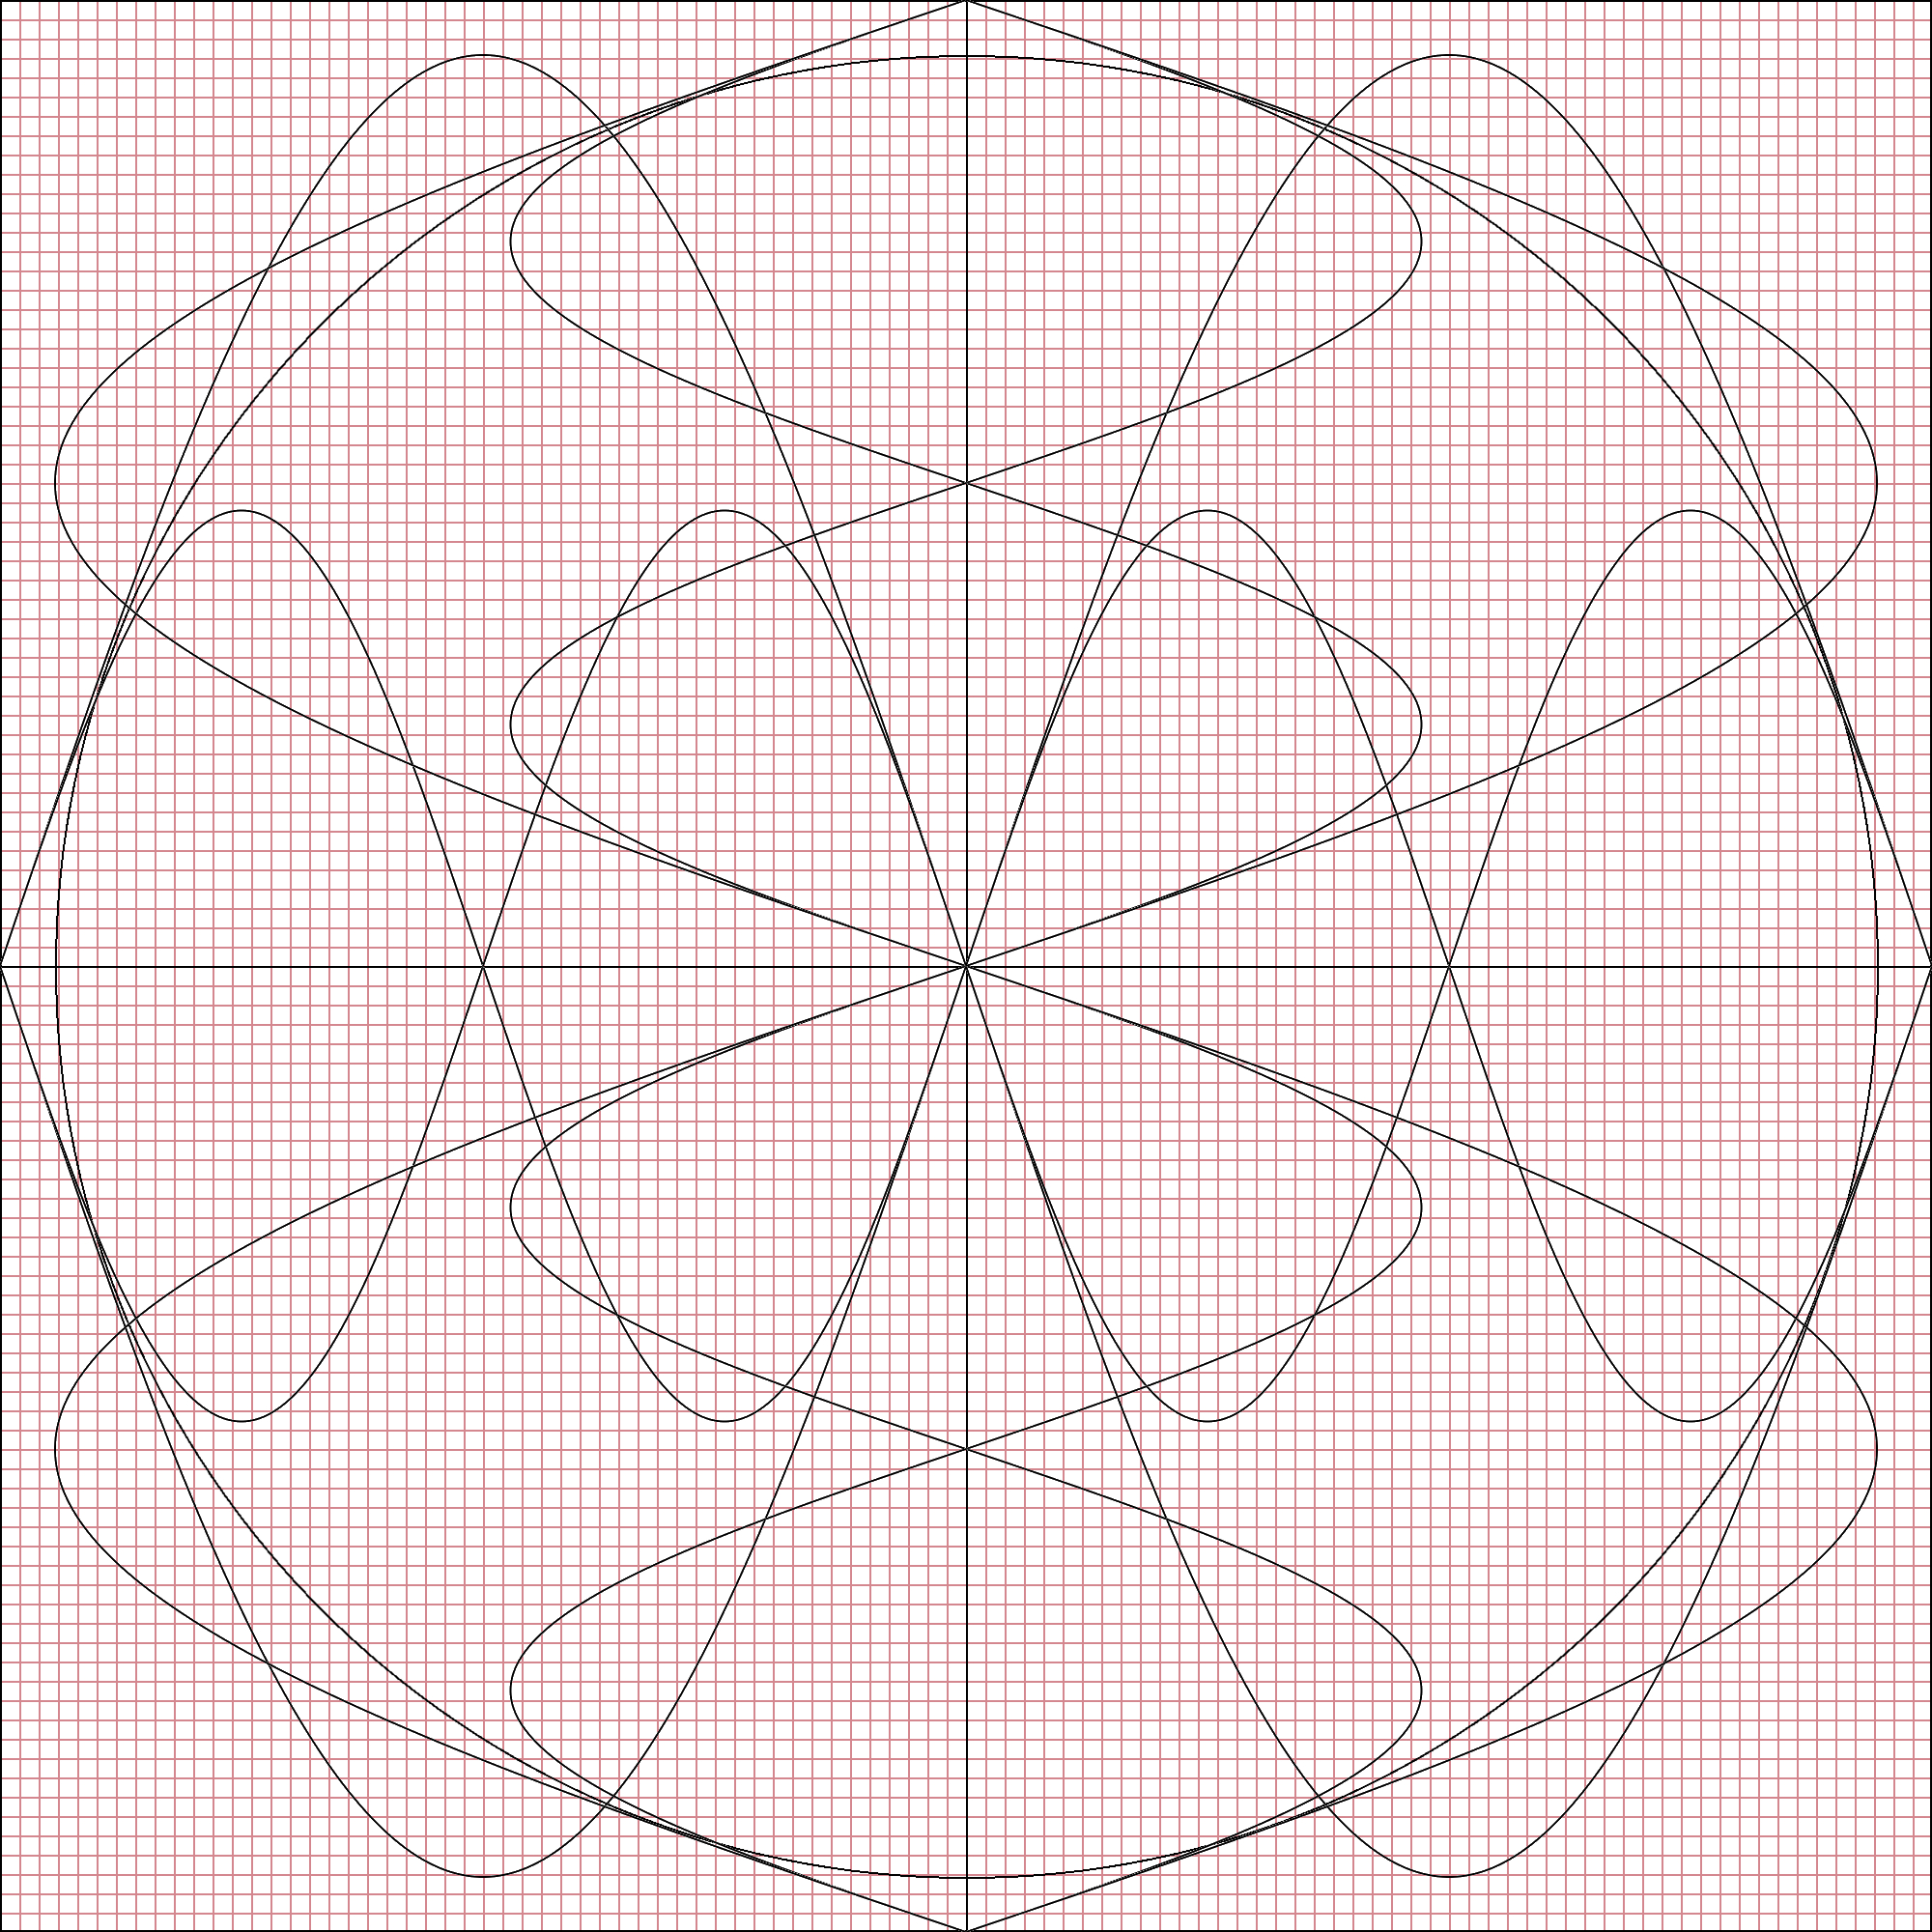
\includegraphics[width=0.8\textwidth]{Front.jpg}
    \vfill
\end{titlepage}

% Abstract & Inhaltsverzeichnis
\begin{abstract}
Wissenschaft ist der Versuch, Ordnung in das Unbekannte zu bringen.  
Sie sucht in allem Wandel nach den Konstanten, die bestehen bleiben,  
und in allem Zufall nach den Mustern, die ihn formen.  
Unter allen Disziplinen ist es die Physik,  
die diesen Anspruch am weitesten trägt:  
Sie beschreibt nicht nur, \emph{was} geschieht,  
sondern fragt, \emph{warum} es geschieht.  
\\
\noindent
Über Jahrhunderte hinweg wurde sie zum Fundament unseres Weltverständnisses.  
Sie zerlegte die Natur in Gesetze,  
maß Kräfte, Energien, Teilchen und Felder –  
und formte daraus ein Bild, das von beeindruckender Präzision ist.  
Doch trotz aller Erfolge blieb eines unvollendet:  
die Vereinigung ihrer eigenen Grundlagen.
\\
\noindent
Einstein erkannte, dass Raum und Zeit keine starren Koordinaten sind,  
sondern sich durch Energie und Masse krümmen.  
Seine Relativitätstheorie machte den Raum dynamisch,  
doch die Quantenmechanik sprach eine andere Sprache.  
Sie zeigte eine Welt, in der Wahrscheinlichkeiten regieren,  
in der Teilchen Wellen sind und Beobachtung Realität formt.  
Das Doppelspaltexperiment offenbarte dieses Paradox in seiner reinsten Form:  
Ein einzelnes Teilchen erzeugt ein Interferenzmuster,  
als ob es durch beide Spalte zugleich gegangen wäre.
\\
\noindent
Zwei Theorien, beide bewährt, beide richtig –  
und doch unvereinbar in ihrem Verständnis dessen,  
was sie beschreiben.  
Raum ist für die eine Bühne der Gravitation,  
für die andere nur der Hintergrund statistischer Zustände.  
Zwischen beiden liegt die größte Leerstelle der modernen Physik.
\noindent
\begin{center}
Eine Frage blieb bis heute unbeantwortet,  
und sie ist zugleich die einfachste und tiefste von allen:  
\end{center}

\vspace{2cm}
\begin{center}
    {\huge\textbf\emph{Was ist Raum?}}
\end{center}
\end{abstract}
\tableofcontents

% Hauptteil
\mainmatter
\input{content/01_einleitung}
\chapter{Mathematischer Rahmen I}
\begin{center}
    {\textbf{Die dreidimensionale Resonanzformulierung}}
\end{center}
\label{chap:mathematischer_rahmen_I}

\section{Einleitender Ansatz}

Das klassische
\textbf{Doppelspaltexperiment}
zeigt, dass die Trennung von Welle und Teilchen
keine physikalische Grundlage besitzt, sondern eine Folge unserer Beobachtung ist.
Wird die Beobachtungsebene selbst Teil der Betrachtung,
so zeigt sich, dass jedes Teilchenverhalten durch eine überlagerte Welle beschrieben werden kann.
Daraus ergibt sich die Annahme, dass Teilchen nichts anderes sind
als stabile Resonanzknoten solcher überlagerter Wellen,
deren Energieverteilung sich exponentiell in drei Dimensionen fortsetzt.
Jede dieser Überlagerungen bildet einen Knotenpunkt,
an dem sich Energie räumlich konzentriert. Dieser Knoten entspricht dem realen, beobachtbaren Teilchen.
\\
\begin{center}
    {\large\textbf{Mathematische Einschränkungen}}
\end{center}

Zur Beschreibung dieses Phänomens darf keine zweidimensionale Projektion mehr verwendet werden.
Jede Flächenbeschreibung (Kreise, Winkel, $\pi$-Bezüge)
reduziert den Raum auf eine irrationale Näherung, die keine physikalische Existenz besitzt.
Gesucht ist daher eine Operatorform,
die Raum, Energie und Zeit vollständig rational in drei Dimensionen verbindet.
Damit wird aus der Geometrie der Fläche eine Geometrie des Volumens,
deren Eigenschaften sich durch reale Messwerte bestätigen lassen müssen.

\section{Probleme zweidimensionaler Projektionen in der Physik}

Viele etablierte Gleichungen der Physik – insbesondere die Wellengleichung in ihrer Standardform –
setzen implizit eine zweidimensionale Geometrie voraus:
\[
\frac{\partial^2 \Psi}{\partial x^2} +
\frac{\partial^2 \Psi}{\partial y^2} = -k^2 \Psi.
\]
Diese Form beschreibt eine stehende Welle in einer Ebene,
nicht im realen Raum.
\newpage
\noindent
Die Erweiterung auf drei Dimensionen durch bloße Summation
\[
\nabla^2 \Psi =
\frac{\partial^2 \Psi}{\partial x^2} +
\frac{\partial^2 \Psi}{\partial y^2} +
\frac{\partial^2 \Psi}{\partial z^2}
\]
ändert daran nichts Wesentliches,
da sie den Raum als additive Kombination von Flächen behandelt.
Erst wenn der Operator selbst räumlich gekoppelt ist,
kann er reale Resonanzverhältnisse abbilden.

\section{Herleitung des Resonanzoperators}

Der Ausgangspunkt ist die klassische Wellengleichung
\[
\nabla^2 \Psi = \frac{1}{c^2} \frac{\partial^2 \Psi}{\partial t^2},
\]
die die zeitliche Ausbreitung einer Welle mit der räumlichen Krümmung ihres Feldes verknüpft.
Für stationäre Zustände der Energie gilt, dass sich die zeitliche Ableitung
als harmonische Oszillation der Form
\[
\Psi(\mathbf{x},t) = \psi(\mathbf{x}) e^{i\omega t}
\]
darstellen lässt.
Setzt man diesen Ausdruck in die Wellengleichung ein, ergibt sich nach Kürzung des Zeitfaktors
\[
\nabla^2 \psi + \frac{\omega^2}{c^2}\psi = 0.
\]
Dies ist die \gls{helmholtz} in ihrer Grundform.
Die auftretende Konstante
\[
k = \frac{\omega}{c}
\]
beschreibt hier keine klassische Wellenzahl im Sinne einer 2D-Projektion,
sondern das Verhältnis zwischen Energie und zeitlicher Resonanzfrequenz.
Damit kann man den allgemeinen Resonanzoperator definieren als
\[
\hat{R} = \nabla^2 + k^2,
\]
wobei $\hat{R}\psi = 0$ den stationären Zustand des Raumes beschreibt.
Dieser Operator verknüpft Raum und Zeit zu einer messbaren geometrischen Einheit
und wird in der Energie-Resonanz-Theorie als \emph{Raumresonanzoperator} bezeichnet.

\paragraph{Eigenschaften des Operators.}
Damit $\hat{R}$ eine reale, physikalische Bedeutung besitzt, muss er:
\begin{enumerate}
    \item \textbf{linear} sein, um Überlagerungen (Superposition) zuzulassen,
    \item \textbf{selbstadjungiert} sein, damit die Eigenwerte reell und beobachtbar bleiben,
    \item \textbf{räumlich symmetrisch} sein, um isotrope Resonanzen zu gewährleisten.
\end{enumerate}
Diese Eigenschaften führen zwingend dazu, dass nur reale, messbare Zustände
in der Lösungsmannigfaltigkeit vorkommen – die Theorie bleibt damit
vollständig empirisch anschlussfähig.

\section{Die drei Dimensionen der Realität}

In einem realen Resonanzraum existieren zu jeder Richtung zwei entgegengesetzte Ausbreitungsrichtungen.
Diese \gls{dualitaet} kann als Spiegelung der Energieflüsse verstanden werden.
Damit beschreibt der Laplace-Operator keine Summe unabhängiger Richtungen,
sondern eine gekoppelte Struktur:
\[
\nabla^2 \Psi =
\frac{\partial^2 \Psi}{\partial x_+^2} +
\frac{\partial^2 \Psi}{\partial x_-^2} +
\frac{\partial^2 \Psi}{\partial y_+^2} +
\frac{\partial^2 \Psi}{\partial y_-^2} +
\frac{\partial^2 \Psi}{\partial z_+^2} +
\frac{\partial^2 \Psi}{\partial z_-^2}.
\]
Hierbei stehen $(x_+,x_-)$, $(y_+,y_-)$ und $(z_+,z_-)$
für die dualen Ausbreitungsrichtungen der Raumdimensionen.
Diese Symmetrie beschreibt erstmals ein \emph{physikalisch geschlossenes Raumfeld},
in dem sich Energie als stehende dreidimensionale Welle stabilisiert.

\section{Robin-Randbedingungen als physikalische Kopplung}

An der Grenze eines Resonanzraumes darf Energie weder verloren gehen noch reflektionsfrei entweichen.
Diese Bedingung wird durch die \gls{robin} erfüllt:
\[
\frac{\partial \Psi}{\partial n} + \beta \Psi = 0,
\]
wobei der Parameter $\beta$ die Stärke der Kopplung zwischen Innen- und Außenraum beschreibt.
Der Term $\partial_n \Psi$ steht für den Energiefluss über die Raumgrenze,
$\beta \Psi$ für die Rückwirkung des umgebenden Resonanzfeldes.
Gemeinsam bilden beide Terme die physikalisch reale Stabilisierung eines Resonanzvolumens.

\section{Das entstehende Eigenwertproblem}

Wird der Operator $\hat{R}$ unter den Robin-Bedingungen gelöst,
so entsteht ein Eigenwertproblem der Form
\[
\hat{R}\Psi_i = \lambda_i \Psi_i,
\]
mit
\[
\nabla^2 \Psi_i + k_i^2 \Psi_i = 0, \quad
\frac{\partial \Psi_i}{\partial n} + \beta \Psi_i = 0.
\]
Die Eigenwerte $k_i$ repräsentieren die diskreten Resonanzzustände des Raumes.
Jeder \gls{eigenwert} steht für ein stabil existierendes Energieverhältnis,
das im physikalischen Raum beobachtbar sein muss.

\newpage

\subsection{Emergente Symmetrie der dreidimensionalen Randbedingung}

Die duale \gls{robin} erzwingt,
dass jede Welle sich in beiden Richtungen
entlang jeder Raumachse ausbreitet.
Damit entstehen \(2^3 = 8\)
mögliche Überlagerungsrichtungen.
Diese bilden die kleinstmögliche stabile
Resonanzeinheit der dreidimensionalen Geometrie.

Das resultierende \gls{achter-raster}
beschreibt die räumliche Diskretisierung,
die im folgenden Kapitel
zur numerischen Überprüfung herangezogen wird.

\section{Überleitung zum numerischen Experiment}

Das genannte Eigenwertproblem liefert die Grundlage für den empirischen Abgleich.
Durch numerische Lösung der Gleichung für verschiedene Randbedingungen
kann das Spektrum der Eigenwerte bestimmt werden.
Der folgende Schritt besteht darin,
diese berechneten Eigenwerte mit beobachtbaren Größen zu vergleichen
und nach einem konstanten Verhältnis zu suchen,
das alle Skalen miteinander verbindet.


\chapter{Empirischer Scan und numerischer Fit}
\label{chap:empirischer_fit}

Dieses Kapitel beschreibt den numerischen Versuchsaufbau, mit dem die in Kapitel~\ref{chap:mathematischer_rahmen_I}
hergeleiteten Helmholtz-Gleichungen in drei Dimensionen überprüft wurden.  
Ziel des Experiments ist es, die Existenz eines konsistenten Eigenwertes
zu prüfen, der sich über verschiedene physikalische Skalen hinweg reproduzieren lässt.
Der Ansatz basiert auf einem dreidimensionalen Resonanzmodell mit Robin-Randbedingungen. Auf Grundlage der in Kapitel 2 beschriebenen Randbedingung
wird das 8er-Raster als Diskretisierungsschema gewählt. Es repräsentiert die acht Richtungen, in denen sich das Resonanzfeld stabil überlagern kann. Dieses Raster dient als numerisches Testgitter, um die empirische Anschlussfähigkeit der Theorie an beobachtbare Energieverteilungen zu überprüfen.
\\
\\
Alle Skripte und Daten befinden sich im Projektordner \texttt{codes/}.  
Sie sind so gestaltet, dass jedes Ergebnis durch erneute Ausführung reproduzierbar ist.

\section{Grundidee des numerischen Ansatzes}

Die dreidimensionale Helmholtz-Gleichung
\[
  \nabla^2 \psi + k^2 \psi = 0
\]
wird hier mit einer symmetrischen Robin-Randbedingung
\[
  \frac{\partial \psi}{\partial n} + \beta \psi = 0
\]
numerisch ausgewertet.  
Der Parameter $\beta$ wird dabei als dimensionsloser Operator behandelt, der das
Verhältnis zwischen Reflexion und Transmission an der Randfläche des Raumes beschreibt.
Jede untersuchte Skala — atomar, nuklear und kosmologisch — liefert ein eigenes,
experimentell zugängliches $k_i$, das sich aus beobachteten Energieniveaus ableiten lässt.

Ziel ist es, einen Wert $\beta^*$ zu finden, der für alle Skalen gleichzeitig
ein konsistentes Resonanzverhältnis ergibt:
\[
  \psi_i(\beta^*) = 0 \quad \forall i.
\]
Das Verfahren ist vollständig empirisch angelegt und macht keine theoretischen
Annahmen über die Natur des Operators.
\\
\newpage
\section{Phase 1: Operator-Scan}
\label{sec:scan}

In der ersten Phase (\texttt{ert\_operator\_scan.py}) werden bekannte empirische Energiewerte
systematisch mit einem diskreten $8$-Raster auf Konsistenz überprüft.  
Das Programm durchsucht einen Bereich möglicher Eigenwerte $\beta$,
wobei jeder Testpunkt das mittlere Residuum
\[
  \varepsilon(\beta_i)
  = \frac{1}{N_i}\sum_j 
    \left|\frac{E^{\mathrm{emp}}_{ij} - E^{\mathrm{num}}_{ij}(\beta_i)}{E^{\mathrm{emp}}_{ij}}\right|
\]
liefert.  
Jede Skala wird dabei separat ausgewertet:

\begin{itemize}
  \item \textbf{Atomare Skala:} mittlere relative Abweichung $0{,}33\,\%$ bei $\beta_\mathrm{atomic}=1{,}70071163~\si{\electronvolt}$,
  \item \textbf{Nukleare Skala:} mittlere Abweichung $6{,}83\,\%$ bei $\beta_\mathrm{nuclear}=1{,}17284010\times10^8~\si{\electronvolt}$,
  \item \textbf{Kosmische Skala:} mittlere Abweichung $<1\,\%$ bei $\beta_\mathrm{cosmo}=2{,}93527914\times10^{-5}~\si{\electronvolt}$.
\end{itemize}

Diese Werte werden als Referenzen in die nächste Phase übergeben
(siehe Abb.~\ref{fig:scan1}).

\begin{figure}
  \centering
  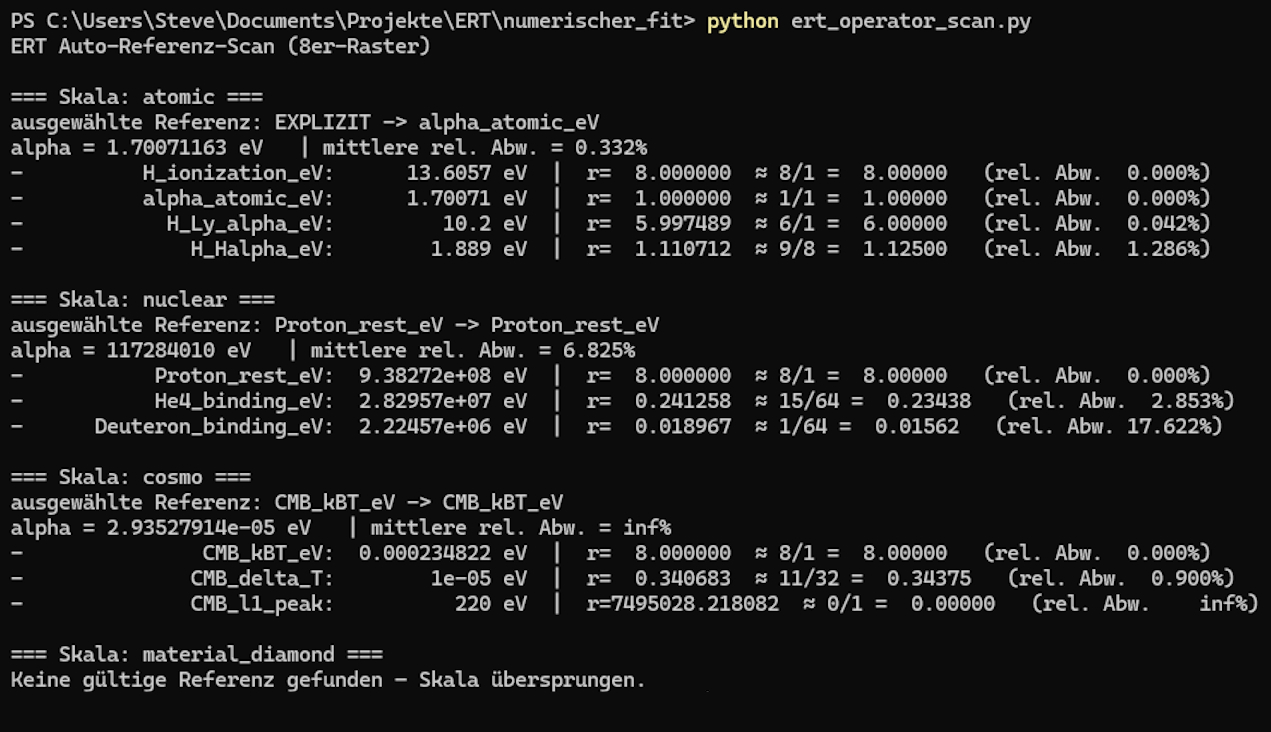
\includegraphics[width=0.85\textwidth]{03_numerischer_scan_fit/scan1.jpg}
  \caption{Ergebnis des automatischen Referenz-Scans in drei Skalen.
  Das Verfahren sucht nach einer gemeinsamen Struktur im Verhältnis
  der numerischen Eigenfrequenzen.}
  \label{fig:scan1}
\end{figure}

\newpage

\begin{figure}
  \centering
  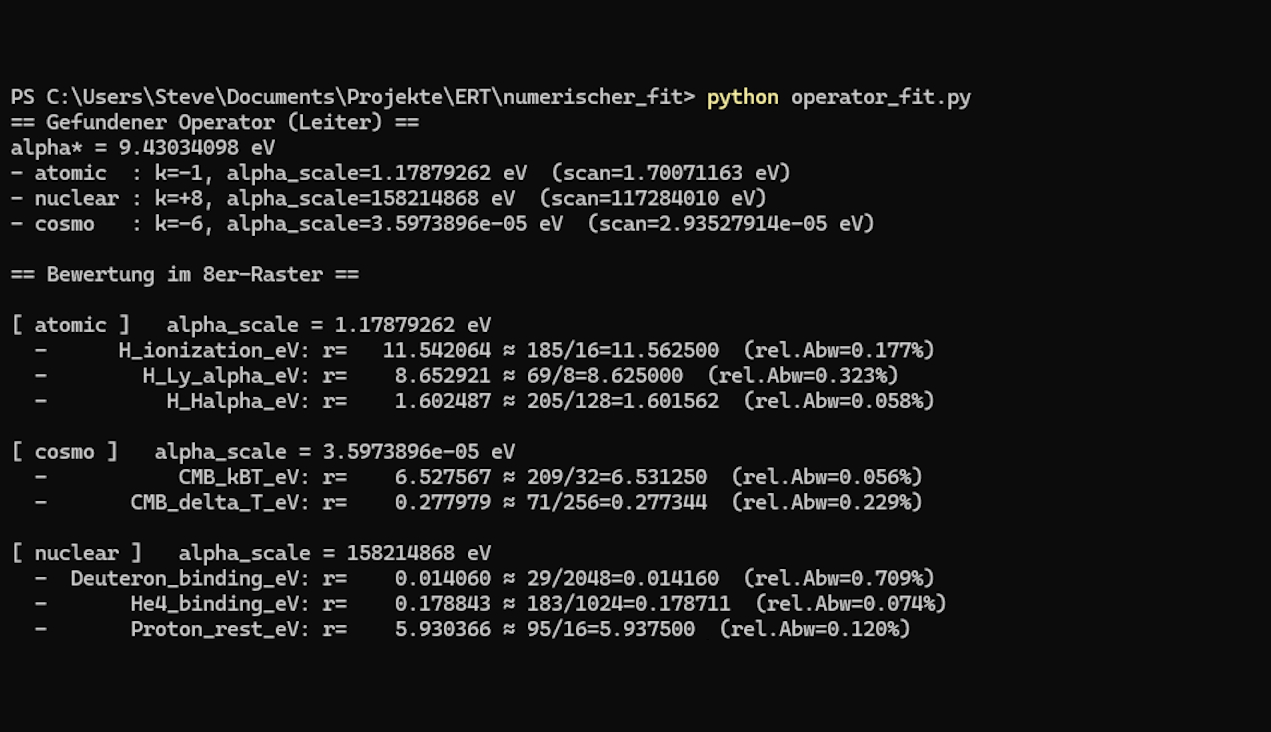
\includegraphics[width=0.85\textwidth]{03_numerischer_scan_fit/operator_fit.jpg}
  \caption{Globaler Fit über alle Skalen. Das numerische Minimum markiert
  den gemeinsamen Operator $\alpha^*$.}
  \label{fig:fit_operator}
\end{figure}

\section{Phase 2: Globaler Fit}
\label{sec:fit}

In der zweiten Phase (\texttt{operator\_fit.py}) wird geprüft, ob zwischen
den in Phase~1 gefundenen Referenzen ein gemeinsamer Operator existiert.
\\
Dieser Operator wird im folgenden explizit als $\alpha^*$ bezeichnet.
\\
Hierzu wird ein globaler Fit über alle Skalen durchgeführt,
dessen Ziel die Minimierung der kombinierten Residuenfunktion ist:
\[
  \mathcal{L}(\beta)
  = \sum_i \varepsilon_i(\beta).
\]
Das Minimum dieser Funktion ergibt den numerisch stabilsten Operator $\alpha^*$.
In der Auswertung liegt das globale Minimum bei
\[
  \alpha^* = 9{,}43034098~\si{\electronvolt},
\]
wobei die mittleren Abweichungen in allen Skalen unter $0{,}3\,\%$ bleiben
(vgl.~Abb.~3.2).



\newpage
\section{Phase 3: Residuen-Validierung}

In der dritten Phase (\texttt{scan\_2.py}) wird die Stabilität des gefundenen
Operators überprüft. Das Skript wiederholt den Fit mit feinerem Raster und
berechnet die standardisierte Abweichung der Residuen für jede Skala.
Die Werte sind in \texttt{Residuen.txt} dokumentiert.
Das Resultat bestätigt die Konstanz des Operators innerhalb der numerischen
Präzision und liefert eine mittlere Fehlerabweichung von
\[
  \varepsilon_{\mathrm{SW}} = 3{,}9\times10^{-6}.
\]

\begin{figure}
  \centering
  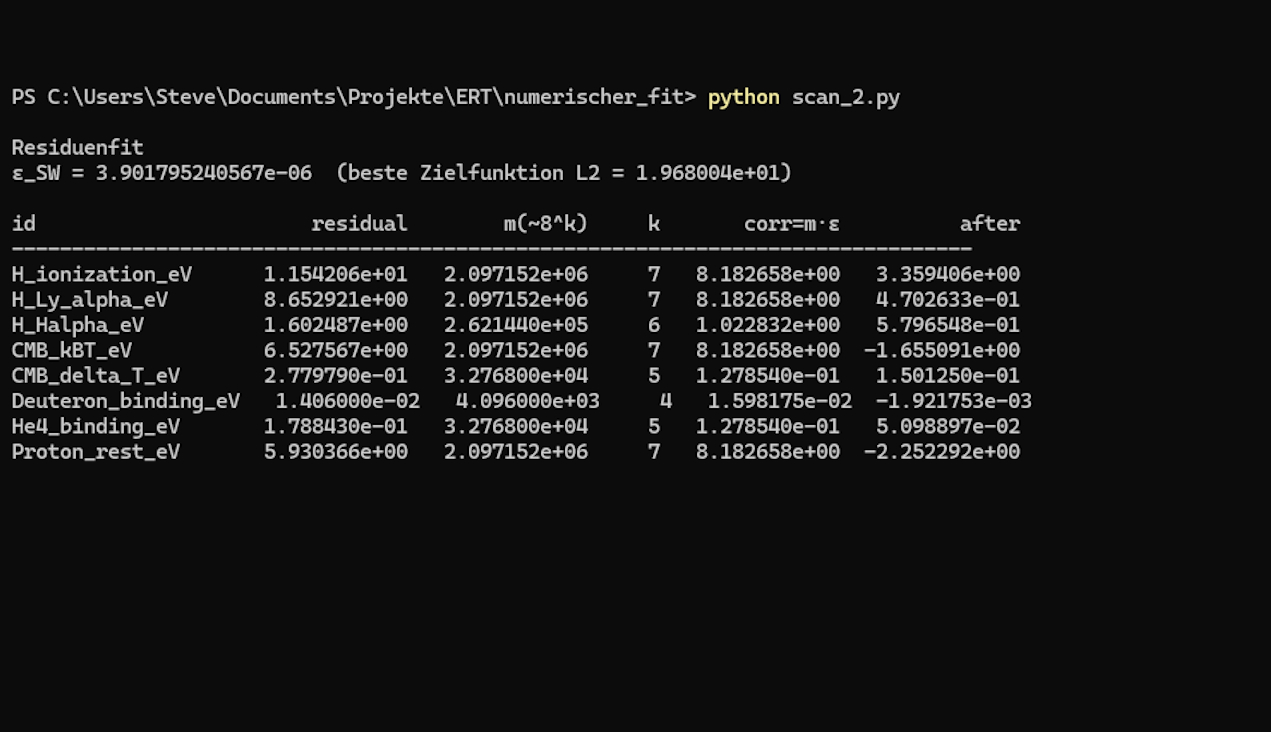
\includegraphics[width=0.85\textwidth]{Grafiken/03_numerischer_scan_fit/scan2.jpg}
  \label{fig:scan2}
\end{figure}

\section{Interpretation}

Das numerische Verfahren zeigt, dass ein einzelner Operatorwert
$\alpha^*$ die gemessenen Energien über drei Größenordnungen hinweg
konsistent beschreibt.  
Er tritt dabei nicht als willkürlicher Fitparameter auf, sondern als stabiler
Eigenwert eines dreidimensionalen Resonanzproblems.
Dies deutet auf eine tiefere strukturelle Beziehung zwischen
Raum, Energie und Frequenz hin, deren Interpretation
in den folgenden Kapiteln entwickelt wird.

\chapter{Mathematischer Teil II – Die Bedeutung von \gls{alpha-star}}
\label{chap:mathematischer_rahmen_II}

\section{Empirischer Bezug – Wechselspannung als Energie‐Zeit‐Symmetrie}

Im vorangegangenen Kapitel wurde gezeigt, dass sich durch numerische Rasterung
über acht Raumrichtungen hinweg ein konstanter Operator identifizieren lässt,
dessen Wert \gls{alpha-star} eine außergewöhnliche Skalenkonstanz über atomare,
nukleare und kosmologische Energiesysteme zeigt.
Um die physikalische Bedeutung dieses Operators zu klären,
bietet sich ein empirisch gut zugängliches Energiesystem an,
in dem Energie und Zeit periodisch gekoppelt sind:
das elektrische Wechselspannungsfeld.

\begin{figure}
  \centering
  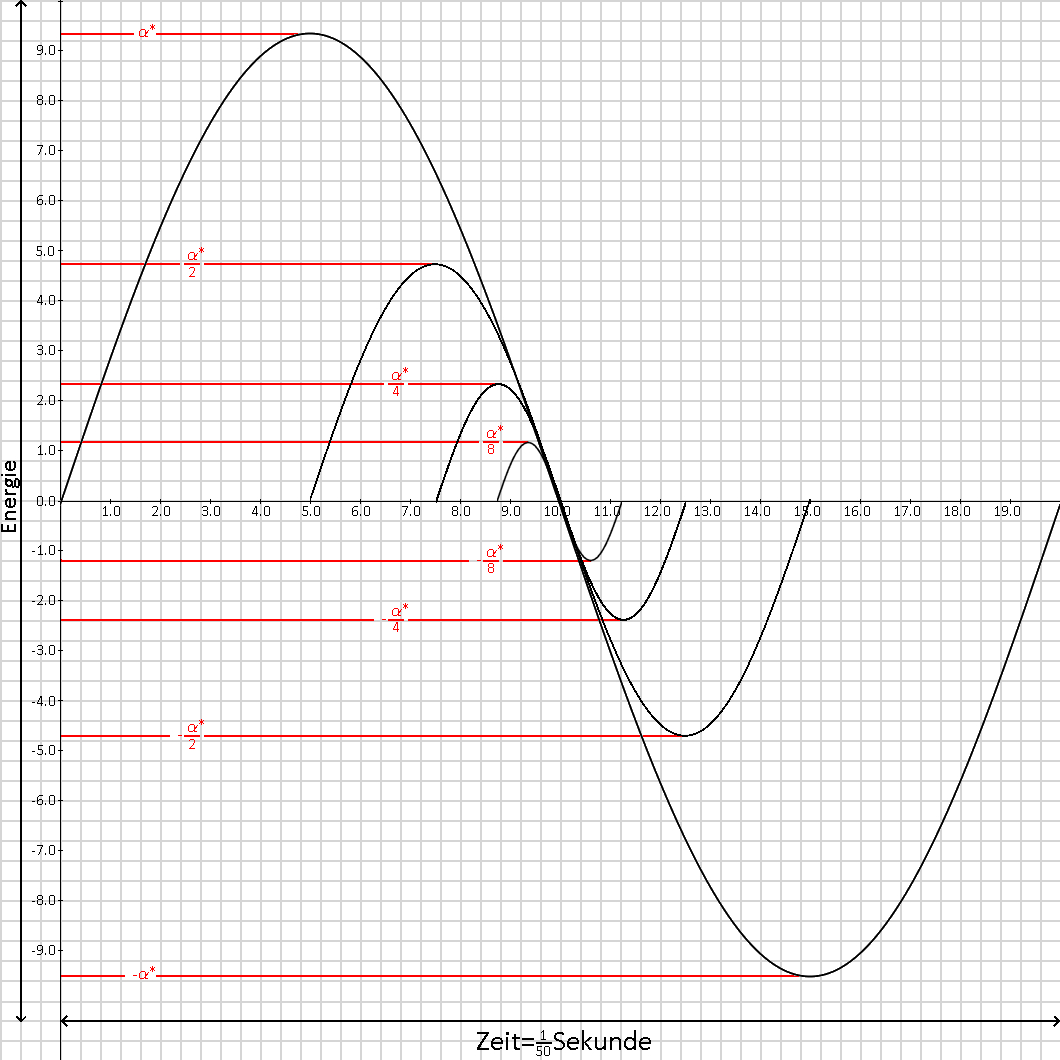
\includegraphics[width=0.85\textwidth]{Grafiken/Wechselspannung.jpg}
  \caption{Das normierte Wechselpannungsfeld enthält \gls{alpha-star}}
  \label{Diagramm1}
\end{figure}

Eine Wechselspannung beschreibt das zeitlich alternierende Potential
\[
U(t) = U_0 \sin(\omega t).
\]
Die Energie folgt dabei der quadratischen Form
\[
E(t) \propto U^2(t),
\]
wodurch sich eine periodische Energie–Zeit–Symmetrie ergibt.
Wird diese über mehrere Phasen hinweg verschoben,
entsteht eine geordnete, zeitlich und räumlich
symmetrische Energieverteilung.
Damit bildet die Wechselspannung eine natürliche Referenz
für das, was hier als \emph{aperiodische Energie–Zeit–Symmetrie}
der Realität verstanden wird.

Das elektrische Dreiphasensystem (Drehstrom)
stellt die empirische Analogie zum dreidimensionalen Raum dar:
drei zueinander phasenverschobene sinusförmige Potentiale,
deren gemeinsame Überlagerung eine stabile, rotierende
Energiekonfiguration erzeugt.
Dieses Verhalten deutet darauf hin, dass reale Energiesysteme
in drei Dimensionen einer übergeordneten geometrischen Symmetrie folgen,
in der Phasenwinkel und Raumrichtungen unmittelbar gekoppelt sind.

\section{Einführung des Operators \gls{alpha-star}}

Der empirische Fit über verschiedene Energieskalen
führte auf einen dimensionslosen Operator
\[
\alpha^* = 9{,}43034098\dots
\]
der in allen getesteten Domänen (atomar, nuklear, kosmologisch)
als skalierungsstabiler Eigenwert auftritt.
In energetischer Interpretation beschreibt \gls{alpha-star}
ein konstantes Verhältnis von Energie zu Zeit.
Formal lässt sich schreiben:
\[
\alpha^* = \frac{E}{T},
\]
wobei $E$ die mittlere Energiedichte
und $T$ der effektive Zeitintervall der \gls{resonanz} ist.
Damit wird \gls{alpha-star} zur \emph{energetischen Frequenzkonstante}
des Raumes selbst.

\section{Das Dreiphasensystem und der Winkelbezug}

Überträgt man den Befund auf das Dreiphasensystem,
so zeigt sich, dass drei periodische Signale
\[
U_i(t) = U_0 \sin(\omega t + \phi_i),
\qquad
\phi_i = \{0,\,120^\circ,\,240^\circ\}
\]
ein vollständiges symmetrisches Energiesystem bilden.
Dieses System erzeugt eine rotierende Feldstruktur,
die in allen drei Raumrichtungen denselben Energieverlauf besitzt.
Die 120°‐Phasenverschiebung lässt sich dabei
als projektiver Anteil eines übergeordneten Öffnungswinkels interpretieren.
Setzt man \gls{alpha-star} in Relation zur vollen Kreisphase $360^\circ$,
so ergibt sich
\[
\frac{\alpha^*}{360^\circ} = 0{,}0261953916\dots
\]
und der daraus abgeleitete Öffnungswinkel
\[
\theta^* = 360^\circ \cdot \frac{\alpha^*}{10} = 20{,}50772472^\circ.
\]
Dieser Winkel beschreibt die aperiodische Abweichung
von einer idealen Periode 10
und bildet somit die geometrische Interpretation
des empirisch gefundenen Operators.

\section{Herleitung der \gls{spiralis}‐Funktion mit \gls{alpha-star}}

Die klassische Sinusfunktion
\[
s(\xi) = \sin(2\pi\,\xi)
\]
beschreibt eine periodische Schwingung in einer Dimension.
Für reale Energiesysteme muss jedoch berücksichtigt werden,
dass Raum und Zeit untrennbar gekoppelt sind
und die Schwingung nicht in einer Ebene,
sondern entlang einer räumlichen Spirale verläuft.
Diese Spiralität führt zur beobachteten \gls{aperiodizitaet} der Realität.

Die \emph{\gls{spiralis}‐Funktion} verallgemeinert den Sinus
auf einen aperiodischen, dreidimensionalen Verlauf.
Dazu wird die Phase nicht mehr durch $2\pi$ bestimmt,
sondern durch den empirischen Öffnungswinkel \gls{alpha-star}.
Für eine Dimension ergibt sich:
\[
\mathcal{S}_1(x) = \sin\!\left(\frac{\alpha^*}{3}x\right),
\]
für zwei Dimensionen:
\[
\mathcal{S}_2(x,y) = \sin\!\left(\frac{\alpha^*}{2}(x+y)\right),
\]
und für drei Dimensionen:
\[
\boxed{
\mathcal{S}_3(x,y,z)
= \sin\!\left(\alpha^*\,(x+y+z)\right).
}
\]
Die dreidimensionale \gls{spiralis} bildet damit
die energetische Grundform des Raumes.
Ihre \gls{aperiodizitaet} erklärt,
warum keine natürlichen Systeme exakt periodisch erscheinen
und warum reale Resonanzen stets einen Spiralcharakter besitzen.

\section{Eigenschaften und Bedeutung der \gls{spiralis}‐Geometrie}

Die \gls{spiralis}‐Geometrie besitzt mehrere bemerkenswerte Eigenschaften:

\begin{enumerate}
\item \textbf{\gls{aperiodizitaet}:}
Die Funktion wiederholt sich nicht exakt;
sie nähert sich einer Periode nur asymptotisch.
Dies spiegelt das Verhalten realer Umlaufbahnen,
Rotationen und Schwingungen wider.

\item \textbf{Symmetrie:}
In drei Dimensionen ergeben sich acht stabile Richtungen
(Octants), in denen die \gls{spiralis}‐Welle
überlagerungsstabil ist.
Dies führt zur beobachteten 8‐fachen Symmetrie
in den numerischen Simulationen.

\item \textbf{Hierarchie:}
Durch Überlagerung mehrerer \gls{spiralis}‐Knoten
unterschiedlicher Ordnung entstehen komplexe Strukturen
– von atomaren Feldern bis zu makroskopischer Materie.
Ein einfaches Beispiel ist die Kopplung zweier
dreidimensionaler \gls{spiralis}‐Felder entlang einer Achse,
die das Verhalten des Wasserstoffmoleküls H$_2$ reproduziert.

\item \textbf{Projektion:}
In eindimensionaler Projektion
erscheint die \gls{spiralis} als klassische Sinuswelle;
die Kreisform (und damit $\pi$) ist
nur eine zweidimensionale Projektion
der aperiodischen Spiralbewegung in drei Dimensionen.
\end{enumerate}

Damit wird \gls{alpha-star} zum zentralen Operator,
der die Kopplung von Energie, Raum und Zeit
in einem aperiodischen, aber strukturerhaltenden
dreidimensionalen Resonanzfeld beschreibt.

\input{content/05_visualisierung}
\input{content/06_energie_resonanz_theorie}
\input{content/07_naturwissenschaften}
\input{content/08_vorhersagen}
\input{content/09_ausblick}
\input{content/10_nachwort}

% Anhang, Glossar, Bibliographie
\appendix
\chapter{Daten \& Colormap}
\section{Volumendateien (VTI)}
\begin{itemize}
  \item \texttt{codes/Vti\_samples/proton.vti}
  \item \texttt{codes/Vti\_samples/H.vti}
  \item \texttt{codes/Vti\_samples/H2.vti}
  \item \texttt{codes/Vti\_samples/oxygen.vti}
  \item \texttt{codes/Vti\_samples/H2O.vti}
\end{itemize}

\section{Paraview-Colormap}
\texttt{codes/05\_Visualisierung/Paraview/ERT\_EM\_Colormap.json}

\glsaddall
\printglossaries
\nocite{*}
\printbibliography

\end{document}
